\section{Simulation}
\label{sec:Simulation}

\begin{figure}
\centering
\subfigure[]{
\centering
    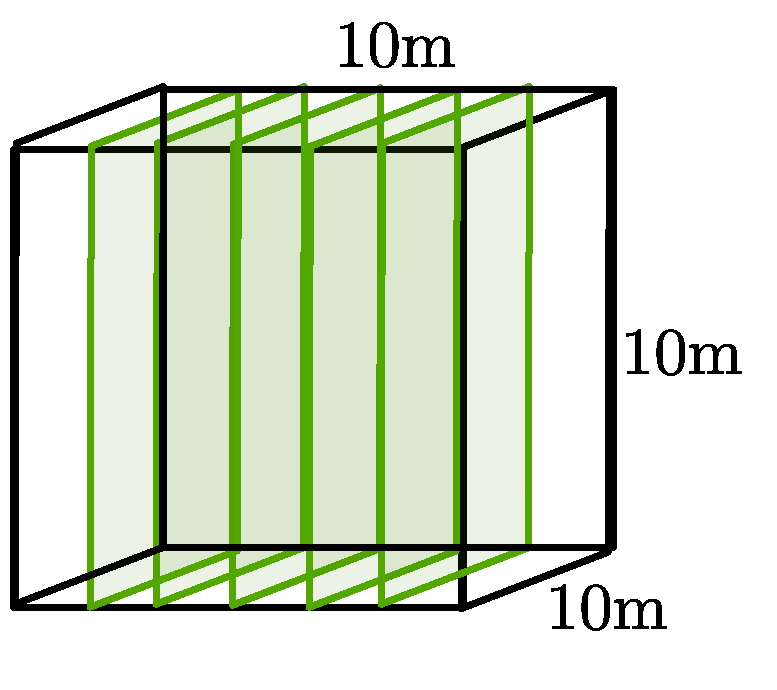
\includegraphics[width=0.5\textwidth]{figs/INT/codexb_nominal_geo.pdf} 
}
\subfigure[]{
\centering
    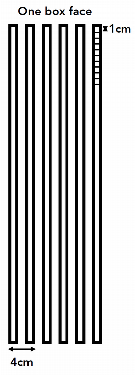
\includegraphics[width=0.15\textwidth]{figs/INT/codexb_box_poc_1.pdf}
}
\caption{\label{fig:nom_geo_cartoon}
    CODEX-b nominal geometry: (a) box showing the $5\times$ inner stations and (b) the 6 layers for the face stations. 
}
\end{figure}


\subsection{Detector Description for High Energy Physics}
As the second part of my project, I developed the simulation framework for both the CODEX-b tracking layers as well as the two-scintillator configuration required for the measurements. We used the Detector Description for High Energy Physics ({\tt DD4hep})~\cite{dd4hep} toolkit for this, in conjunction with {\tt Gauss}, the standard LHCb simulation package. {\tt DD4hep} uses the {\tt ROOT} {\tt TGeometry} class for loading the detector geometry in memory and is being developed for high-luminosity LHC. Further, the project is a software framework to provide overall detector description for experiments. It offers consistent description through a single source of detector information for simulation, reconstruction, conditions (alignment), {\em et al.}, and will be adopted by LHCb for the Upgrade. During my internship, I built the geometry of CODEX-b constructing hierachy system, from scratch. I included the concrete shield wall to block particles generated at the interaction point (IP) from particle gun or minimum bias simulation and also checked for the energy deposits and positions of CODEX-b hits, simulated used {\tt DDG4}, the in-built {\tt GEANT} package for {\tt DD4hep}. 

%I learn how to make geometry: layer, station, super staion, envelope (hierachy).
%I define materials for our detector and CODEX-b geometry such as concrete, Herschel detector.
%Layer consists of silicon, station consists of aluminum. 
%There is a veto cone with two lead and one silicon. 
%Also just in front of CODEX-b, concrete wall exists to veto muons.
%First of all, using muon particle gun with high energy, test our geometry.
%And then using HepMC to generate pp collisions and do the same process as muon particle gun.
%I made hierachy system to build CODEX-b (envelop, super station, station, layer).
%I could check energy deposits and positions of CODEX-b hits.






\subsection{Geometry construction}
The first geometry I constructed was CODEX-b, consisting of two parts, face stations and inner stations. In the nominal version in the proposal~\cite{Gligorov:2017nwh}, there is a face station on each face of the Codex-b box volume, and each face station has 6 layers of resistive plate chambers (RPC) at 4~cm intervals with 1~cm granularity, as shown in Fig.~\ref{fig:nom_geo_cartoon}b. The size of each layer is $10 \times 10$~$m^{2}$ and the thickness is 2~cm. Further, the geometry also included 5 inner stations, as shown in Fig.~\ref{fig:nom_geo_cartoon}a, each containing a triplet of RPC layers. For simplicity, we replaced the RPC's by Silicon tracker layers, and noted the timestamps of the hits in the simulation, since RPC's also provide timing information. We also created a concrete shield wall with 3.2~m thickness, placed just in front of CODEX-b box. In addition, there is a proposed veto cone~\cite{Gligorov:2017nwh} with two lead absorber and one active silicon layer sandwitched in between. Figure~\ref{fig:geo_dd4hep} shows the geometry construction in {\tt DD4hep}. The second geometry comprise two scintillator plates which is the same as our measurement configurations. The plastic material composition in {\tt GEANT} was adopted from HeRSCheL.

%In this simulation we had been implemented layers as a tracker instead of RPCs.
%Inner station also has same configuration except number of layers.
%It will be equally spaced with triplets along the depth to minimize distance between reconstructed vertex and 1st measurement. 

%To make coincidence setup with test-bench, I made two Herschel plates with the same positions where all equipment have set.
%Two plates with 30 x 30~$cm^{2}$ size, 2~cm thickness.
%There is a concrete wall in front of scintillators.
%3~m thickness to suppress particles from pp collisions.
%Roughly in 1000 events, it has hits on scinitillators 4 - 9 events.
%There is a proposed veto cone. It consists of two lead absorbers and one silicon tracker.
%There is also concrete wall which blocks radiations (or particles) to reach CODEX-b box. 
%It has 3.2~m thickness.

\begin{figure}
\centering
\subfigure[]{
\centering
    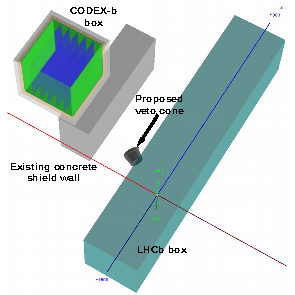
\includegraphics[width=0.47\textwidth]{figs/INT/CODEXbBigGeo.pdf} 
}
\subfigure[]{
\centering
    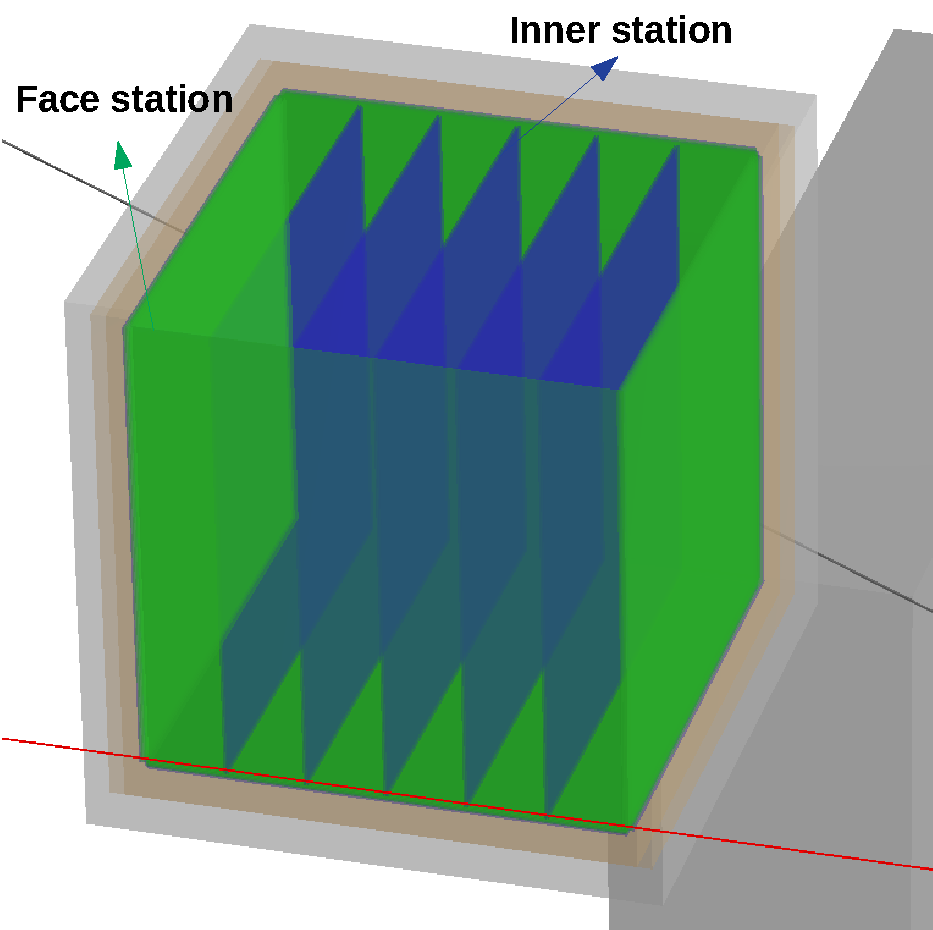
\includegraphics[width=0.47\textwidth]{figs/INT/ZoomVersion.pdf}
}
\caption{\label{fig:geo_dd4hep}
    CODEX-b simulation geometry in {\tt DD4hep}: (a) overall, (b) close-up view. 
}
\end{figure}


\subsection{Simulation status}


\begin{figure}
\centering
\subfigure[]{
\centering
    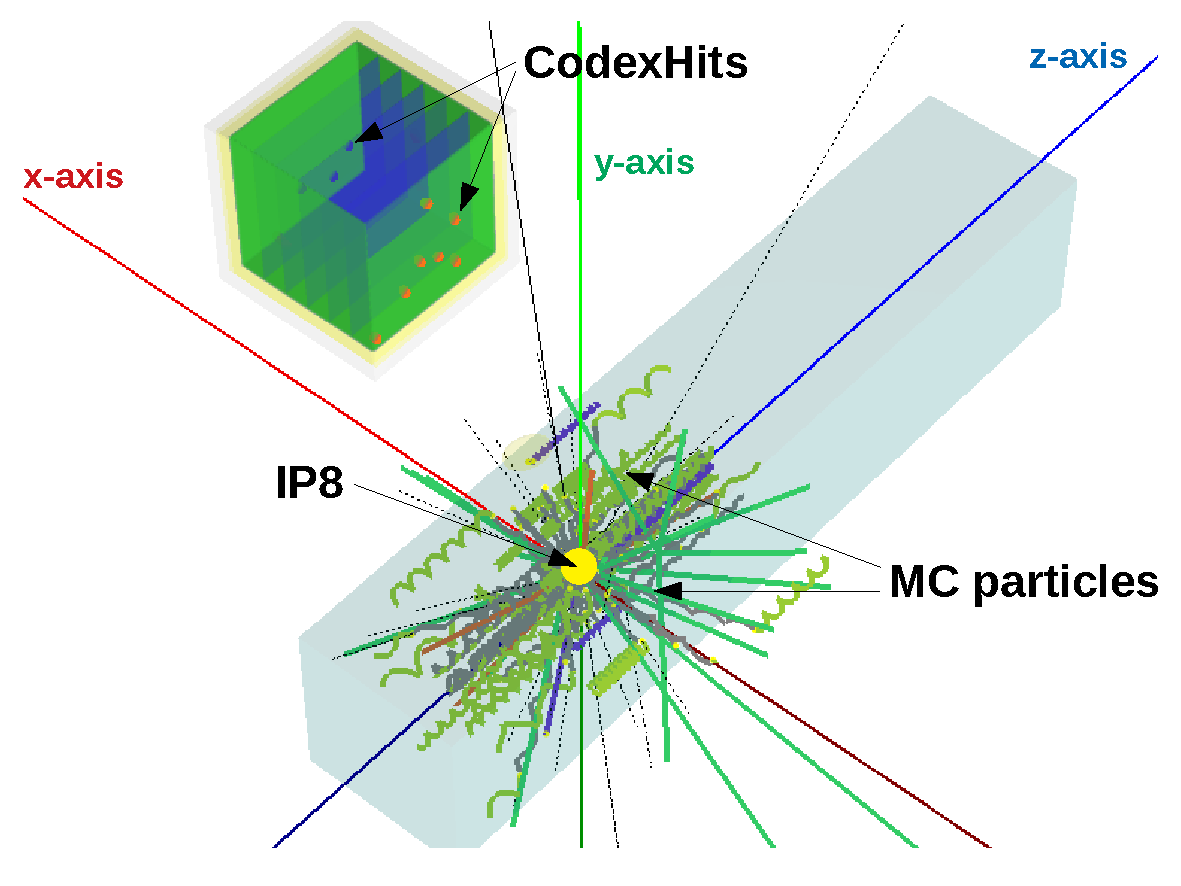
\includegraphics[width=0.75\textwidth]{figs/INT/Minbias.pdf}
}
\subfigure[]{
\centering
    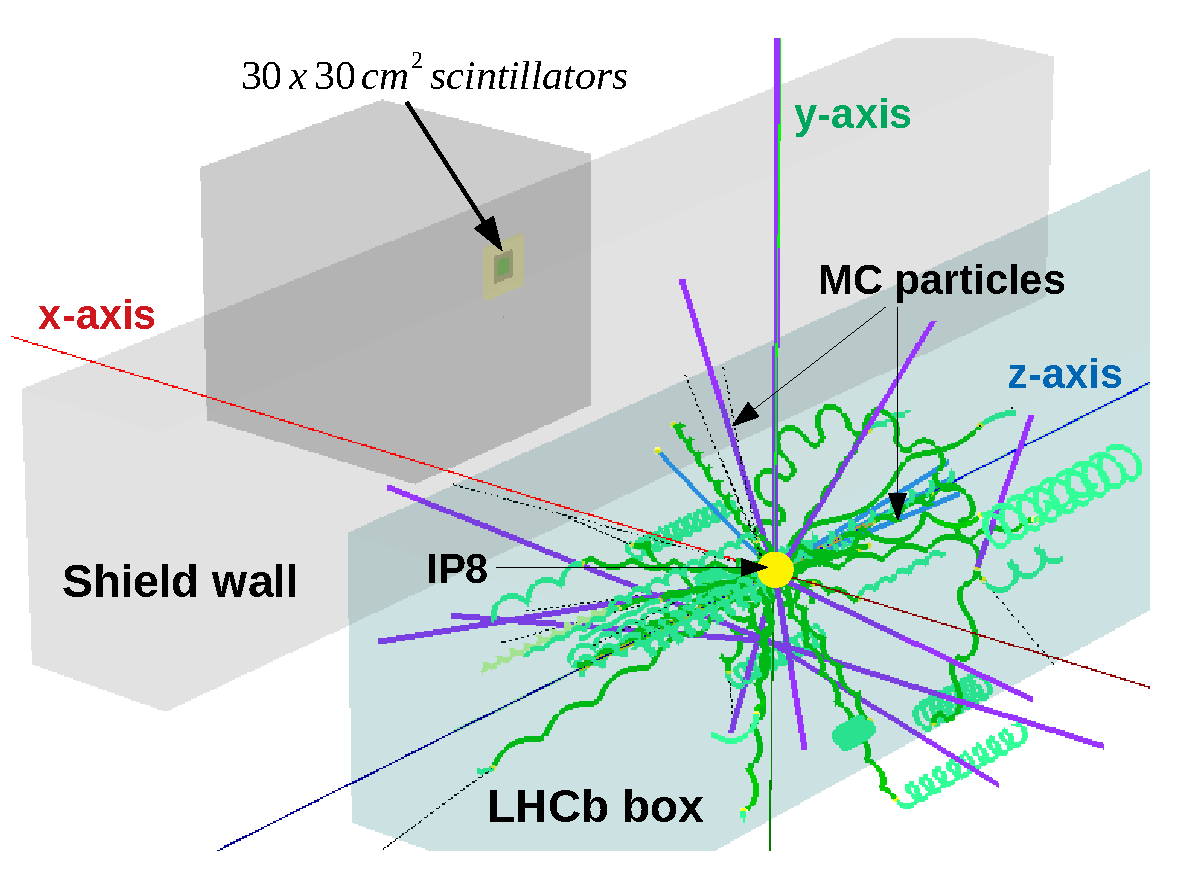
\includegraphics[width=0.75\textwidth]{figs/INT/Scint.pdf}
}
\caption{\label{fig:dd4hep_events}
    Validation of the {\tt DD4hep} based simulation with minimum bias events: (a) CODEX-b box with the shield wall removed, and (b) two-plate scintillators for measurement campaign.}
\end{figure}

As mentioned above, we designed two different detector geometries based on the proposal paper (Codex-b) and the measurement configuration (HeRSCheL scintillators). Both were tested with $\mu$ particle gun generated at 1\tev, and minimum bias events generated in {\tt Gauss} and loaded in {\tt DDG4} using {\tt HepMC} files. 
No hits were recorded in the CODEX-b volume when tested with $32,000$ minbias events with the concrete wall included. Therefore, we decided to remove the shield wall to make sanity checks. Figure~\ref{fig:dd4hep_events}a shows hits from minimum bias events with the concrete wall removed. Figure~\ref{fig:dd4hep_events}b shows the two-scintillator configuration. Again, no hits were recorded at this point, due to the small acceptance, low statistics samples and presence of the contrete wall. However, the geomery setup is validated with these checks.

